
This section is built on our code repository, which is available at \url{GITHUB}.
All the competitive methods are implemented in C, using arbitrary precision arithmetic
and a flow of cryptographic random bits. A part of the implementation is devoted to reproduce our experimental results.
Experiments were conducted on a MacBook Pro (Apple M4 Pro chip, 14-core CPU) with 48GB of unified memory.
%, running macOS 26.6.2.


\subsection{Overview of the experimental approach}

This section evaluates the practical performance of the algorithms introduced in \Cref{sec:algo,sec:gen}
with a focus on measurable scalability limits.
Our evaluation targets five quantities: preprocessing time, sampling throughput, memory footprint, cryptographic random-bit consumption and savings.
First, all computations use exact integer arithmetic, so results are free from
floating-point rounding artifacts. Second, we use highly
compact data structures, which makes explicit the trade-off at the core of our approach:
entropic efficiency (measured in bits) versus time efficiency.

A distinctive feature of our implementations is support for arbitrary precision arithmetic. To the best of our knowledge,
this is the only approach in our comparison that natively provides exact sampling under arbitrary precision.
Random sampling is coupled with a dedicated background thread that continuously refills a bitstream.
This design enables the use of cryptographic random bits, which are expensive to obtain in practice,
with a limited impact on performance, because bit production is decoupled from sampling and overlapped in parallel (the reported times include the CPU time of this thread).
All these features enable scaling in several independent directions: the number of objects can grow
without a fixed-width bound, and the weight of each object can also grow arbitrarily large.
This property is essential for high-precision and large-distribution regimes where fixed-size numeric types become a bottleneck.

Beyond of our new algorithm, we implemented four variants of algorithm provided in the literature:
\textsc{Fldr}, \textsc{Aldr}, Rust-Alias, and Fraction-Alias Samplers, all in arbitrary precision arithmetic.
While these implementations provide exactness and numerical robustness, none of them scales satisfactorily
across all target regimes. The remainder of this section quantifies these limits through a comparative analysis
of memory footprint, preprocessing cost, random-bit consumption, and sampling throughput.


\subsection{Case Study: Combinatorial Chemistry}
\label{sec:chemie}

What is following illustrates how exact sampling becomes essential
when the underlying combinatorial space is too large, as in several nowadays applications.
The chemical space, i.e. the set of all combinatorially plausible stable
molecules, is far too vast to be enumerated. Reference databases report
sizes ranging from $9.7 \cdot 10^{7}$ molecules for the smallest
structures (e.g., GDB-17, up to 17 heavy atoms) to several trillion
compounds for modern make-on-demand combinatorial
libraries~\cite{SSHL26}, and beyond roughly thirty heavy atoms the
number of possible structures far exceeds $2^{64} \approx 1.8 \cdot
10^{19}$. Consequently, any statistical analysis based on a subset of this
space is structurally biased unless the sample is representative of the
true underlying distribution.

To address this context, Monterrubio-Chanca and von Rudorff~\cite{MR25}
proposed a method for producing unbiased, representative samples of
chemical space without ever enumerating it, applicable to molecules containing
on the order of 30 heavy atoms. Obviously, this is a regime in which exhaustive enumeration is
impossible. The method proceeds in five steps:
\begin{enumerate}
  \item Generation of all theoretically possible chemical formulas by
    integer partitioning; %, from valence and stoichiometry constraints;
  \item Grouping of these formulas by degree sequence;
    %, the combinatorial skeleton of the molecular graph, independent of the specific chemical elements involved;
  \item Distinction between ``pure'' and ``non-pure'' sequences, depending
    on whether several elements of the same valence appear;
  \item Estimation of the size of each group, either through exact
    counting or through a heuristic based on the graph's average path length when
    exact counting proves too costly;
  \item Weighted random sampling among the groups, proportional to their
    estimated size, followed by the sampling of a representative molecule
    within the chosen group.
\end{enumerate}
We note that the two steps \textbf{1.} and \textbf{5.} are classical in the context of combinatorics and combinatorial
algorithm design. Especially step \textbf{5.} is a classical application of the Alias method, which is the focus of this paper.
All their results are reproducible through their open-source \texttt{nablachem} Python
package~\cite{nablachem}.

Using their library, we derive the distribution of chemical molecules containing 32 heavy atoms, among Carbon, Hydrogen, Oxygen, Nitrogen, and Fluorine. The total number of molecules is $N = 20\,484$, and the sum of their weights is about $1.25 \cdot 2^{168} \sim 4.7 \cdot 10^{50}$. Thus in the following benchmarks for the sampling method, we used these parameters, which seem representative of the actual combinatorial chemistry research. Remark that step \textbf{5.} cannot be performed without bias in their library based on floating-point arithmetic samplers that are not precise enough in this regime. More details about this case study case be found in our code repository.
%Appendix~\ref{app:chemistry}.


\subsection{Algorithms with arbitrary precision integers}


The goal of these experiments is to compare our approach with existing algorithms for discrete random sampling.
Following the design of our Integer-Alias Sampler, the next phase focuses on an experimental evaluation of our algorithm against existing methods (adapted with arbitrary precision). We start from the code repository of Saad et al.~\cite{SFRM19} in order to add our implementation in their comparison: we thus are able to run all their benchmarks. We have adapted the original memory consumption analysis to the precise size used by the data structures built by the preprocessing step.

% \noteAnt{Dire un mot qu'on a prog en C, avec GMP et que les exp sont faite sur la spec de ma machine,
% dire qu'on a modifié l'analyse de l'espace mémoire que nous ne trouvions pas adéquat pour la comparaison entre preprocessing, qu'on gère une pile d'alea pour se baser sur de l'alea crypto sans ralentir la construction de la simulation}

 While the original implementations by Saad et al. compared several different literature approaches to emphasize random bit consumption, it is more relevant in our context to retain only the top three methods from the literature, according to our efficiency constraints (time, memory, and random bit consumption), while addressing our main challenge of safety at scale via arbitrary-precision arithmetic. Consequently, we compare the following algorithmic approaches:
\begin{itemize}
    \item \textsc{Fldr} Sampler: Saad et al.~\cite{SFRM19} that we adapted for arbitrary-precision integers;
    \item \textsc{Aldr} Sampler: Saad et al.~\cite{DS26}, an improvement of FLDR in the context of random bit consumption, that we also adapted for arbitrary-precision integers;
    \item Rust-Alias Sampler: Rust Developers, a variant of Walker version coded in Rust with integer arithmetic~\cite{Rust25}, where we also have modified types to support arbitrary-precision integers;
    \item Fraction-Alias Sampler: our new exact version of Walker-Alias using exact rational fractions (with arbitrary precision) instead of floating-point numbers;
    \item our Integer-Alias Sampler: our new algorithmic approach, in two implementations sharing the same table. \emph{v1} optimizes random-bit consumption, with Lumbroso's bit-optimal \textsc{Uniform} and \textsc{Bernoulli}~\cite{Lumbroso13}; \emph{v2} optimizes running time, with Lemire's multiply-and-shift \textsc{Uniform}~\cite{Lemire19}, the Bernoulli test reusing the same 64-bit random word, at the cost of 64 random bits per draw.
\end{itemize}

We deliberately leave floating-point samplers (e.g., Walker--Vose with IEEE doubles) out of the comparison:
they are approximate, and here the approximation is not marginal. In 179 of our 201 distributions, some
objects have a share $N w_i / W$ of their bucket below $2^{-53}$, the resolution of a double-precision
threshold (17\,525 of the 20\,484 objects for the median distribution): a floating-point sampler would
never draw them. Its running time would thus be that of another distribution, and is no meaningful
reference; this is precisely the regime our exact samplers are designed for.

The experimental protocol starts by fixing the distribution size (the number of objects), that
we take to be $N = 20\,484$ and the total weight distribution to be the one computed in the context of combinatorial chemistry (see Section~\ref{sec:chemie}) $W \approx 4.7 \cdot 10^{50}$.
The measurements were collected on a set of random distributions following a Dirichlet distribution.
Using a Dirichlet distribution allows varying the entropy while maintaining fixed values for parameters $N$ and $W$. The distribution itself is not of major importance, once we can choose for the average weight of an object or the entropy of the resulting random distribution (e.g. a gaussian distribution of weights would have given the same kind of experimental simulations).
The observed entropy corresponds to Shannon entropy. The latter is a central theoretical measure
in the context of random sampling. We refer the reader to the seminal paper of
Knuth and Yao~\cite{KY76} for a general overview. Essentially, we note that the closer a distribution is to a uniform distribution, the higher its entropy (bounded by $\log_2(N)$).
Conversely, a strongly biased distribution (e.g., one element with a very large weight and many elements with a weight of $1$) results in lower entropy.
For each distribution, among the 200 random ones, 10 millions of objects have been sampled to measure the average sampling time and the average number of random bits consumed.

\begin{figure}[htb]
    \centering
    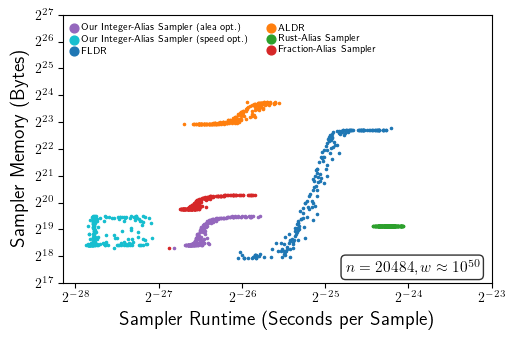
\includegraphics[width=0.48\textwidth]{figs/Runtime-memory.png}
    \hfill
    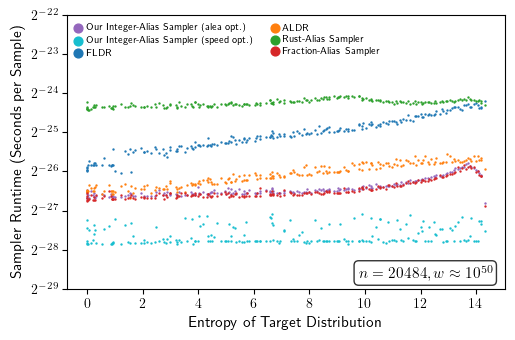
\includegraphics[width=0.48\textwidth]{figs/Entropy-runtime.png}
    \caption{Sampling runtime of the compared algorithms under arbitrary precision, against the memory footprint (left) and the entropy of the distributions (right)}
    \label{fig:runtime_memory}
\end{figure}

Figure~\ref{fig:runtime_memory} (left) plots the runtime of the sampling step against the memory footprint of the internal data structures, with each dot corresponding to one random distribution (averaged over 10 million samples). Remark that $2^{-20}\text{s} = 0.95\,\mu\text{s}$ and $2^{20}\text{B} = 1\text{MB}$. Beyond individual algorithm comparisons, the spread of each cluster is informative: the tight horizontal grouping of Alias-based methods reflects a fundamental algorithmic property, namely that their $O(1)$ sampling step is structurally independent of the target distribution, so every input distribution yields essentially the same runtime. By contrast, \textsc{Fldr} and \textsc{Aldr} exhibit a much wider horizontal spread, exposing their sensitivity to the shape of the distribution. The resulting picture traces an implicit Pareto frontier in the (runtime, memory) plane: \textsc{Fldr} and \textsc{Aldr} occupy the fast-but-memory-intensive region for favorable distributions, while Alias-based approaches occupy the compact-and-predictable region. Within the Alias family, our Integer-Alias Sampler consistently shifts the cluster to the left of Rust-Alias at comparable memory cost, demonstrating that integer normalization by $\mathtt{cs}$ rather than by the full cumulative weight $W$ produces a concrete speedup in the sampling step, independently of the distribution. Its v2 implementation is the fastest of all compared samplers, about $2.3$ times faster than v1 (median over the distributions).

Let us now make the entropy explicit as an independent variable to understand its role in the runtime, memory footprint, and preprocessing time.

\begin{figure}[ht]
    \centering
    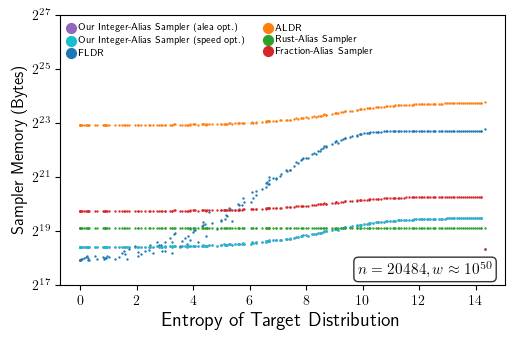
\includegraphics[width=0.48\textwidth]{figs/Entropy-memory.png}
    \hfill
    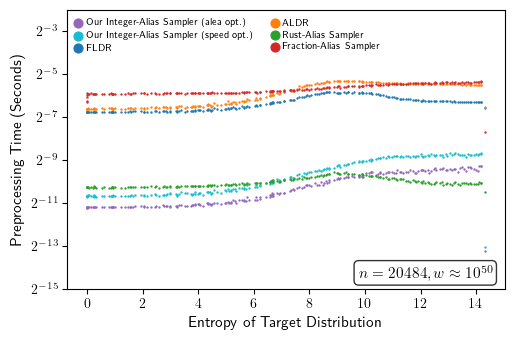
\includegraphics[width=0.48\textwidth]{figs/Entropy-preprocessing.png}
    \caption{Memory footprint (left) and preprocessing time (right) of the compared algorithms under arbitrary precision, as a function of the entropy of the distributions}
    \label{fig:memory_preprocessing}
\end{figure}

Figure~\ref{fig:runtime_memory} (right) confirms that Alias-based runtimes are near-constant across the full entropy spectrum. This invariance is not merely an empirical regularity: it is a direct consequence of the preprocessing step encoding the entire distribution into the alias table, so that each draw requires only a uniform bucket selection and a single Bernoulli test, regardless of the distributional complexity. The entropy-dependence of \textsc{Fldr} and \textsc{Aldr} has a different, more fundamental cause: both algorithms are built on the DDG-tree framework of Knuth and Yao~\cite{KY76}, in which random bits are consumed one at a time to navigate a binary decision tree. The expected number of bits per draw is approximately equal to the Shannon entropy of the distribution, and since each bit operation carries a fixed cost, the average runtime scales accordingly. As a result, \textsc{Fldr} and \textsc{Aldr} are \emph{faster} at low entropy (skewed distributions produce short, predictable tree paths) and \emph{slower} as entropy increases toward $\log_2(N)$ (near-uniform distributions require paths of maximal depth). The crossover at roughly half the maximum entropy (beyond which our Integer-Alias Sampler outperforms \textsc{Aldr} in runtime) reflects the point where the entropy-proportional cost of \textsc{Aldr} exceeds the constant cost of the Alias approach. The combinatorial chemistry application of Section~\ref{sec:chemie}, with its strongly skewed weight distribution falls in the low-entropy regime where \textsc{Fldr} and \textsc{Aldr} are at their most competitive; yet even there, our Integer-Alias Sampler remains within the same order of magnitude in runtime while providing strictly superior memory efficiency.

Regarding memory (Figure~\ref{fig:memory_preprocessing}, left), Alias-based approaches are more compact than \textsc{Aldr} across all entropies, and than \textsc{Fldr} except at low entropy, where its tree is small. Note that we report the exact memory footprint of the data structure produced by the preprocessing step. Within the Alias family, two observations are worth noting. First, even though the integer weights used by the Rust-Alias Sampler are $N$ times larger in value than those of our Integer-Alias Sampler (since Rust takes the total weight $W$ as the target cell capacity rather than $\mathtt{cs}$) the resulting table requires at most one additional cell, so both approaches yield similar memory footprints. Ours nevertheless grows with the entropy: our table stores each threshold with its significant bytes only, and the thresholds of light objects get longer as the distribution flattens. This confirms that the runtime advantage of Integer-Alias observed in Figure~\ref{fig:runtime_memory} (left) stems from the arithmetic cost of the Bernoulli step on large integers, not from a cache or layout effect. Second, the Fraction-Alias Sampler's table is approximately twice as large as those of the other Alias approaches: this is a direct consequence of storing exact rational numbers (numerator and denominator in arbitrary precision) rather than a single integer per entry, and it quantifies the memory cost of the more general rational representation.

Figure~\ref{fig:memory_preprocessing} (right) reports the preprocessing time, i.e., the construction of the data structure from the weights, file parsing excluded (for \textsc{Fldr}, whose construction is written in Python in~\cite{SFRM19}, we use a C port producing the same encoding). Our Integer-Alias Sampler, together with Rust-Alias, has the cheapest preprocessing: below $2.5$\,ms on every distribution, about twenty times less than \textsc{Fldr}, \textsc{Aldr} and the Fraction-Alias Sampler ($10$ to $25$\,ms). It only performs a linear number of integer operations on the weights, whereas \textsc{Fldr} and \textsc{Aldr} scan the binary expansion of every weight at each level of their DDG tree, and Fraction-Alias normalizes a rational number after each operation.

\begin{figure}[ht]
    \centering
    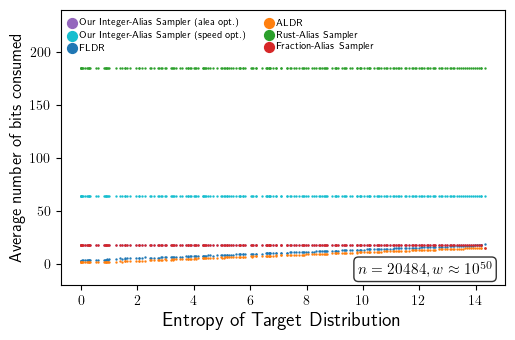
\includegraphics[width=0.48\textwidth]{figs/Entropy-bits.png}
    \hfill
    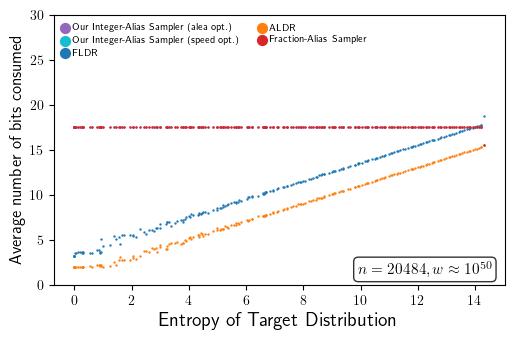
\includegraphics[width=0.48\textwidth]{figs/Entropy-bits2.png}
    \caption{Randomness consumption of the compared algorithms under arbitrary precision, as a function of the entropy of the distributions. The right plot zooms into the left one, capping the vertical axis at 30 bits}
    \label{fig:entropy_bits}
\end{figure}

Figure~\ref{fig:entropy_bits} reports the average number of random bits consumed per sample. The rightmost plot zooms into the leftmost one by capping the vertical axis at 30 bits, excluding Rust-Alias, whose consumption is an order of magnitude higher, and our v2 implementation ($64$ bits per draw). This anomaly has a structural cause: instead of sampling a Bernoulli variable, in the Rust approach requires drawing a uniform integer in $[0, W)$ where $\log_2(W) \approx 153$ bits (far beyond the $\log_2(N) \approx 14$ bits needed by our Integer-Alias Sampler). This is the direct price of the absence of weight normalization in the Rust implementation, and it renders that approach impractical for large-precision regimes regardless of its time efficiency.

Among the remaining four algorithms, \textsc{Fldr} and \textsc{Aldr} consume fewer random bits than our Integer-Alias Sampler across all entropies, with \textsc{Fldr} achieving the information-theoretic optimum of Knuth and Yao~\cite{KY76}. However, this entropic advantage narrows as entropy increases. In the high-entropy regime (distributions close to uniform), the dominant cost for any sampler is the uniform bucket selection, which requires $\log_2(N)$ bits regardless of the algorithm. As the distribution approaches uniform, this fixed cost dominates, and the overhead of our Integer-Alias Sampler relative to the optimum becomes negligible. In this limit, our algorithm thus simultaneously achieves $O(1)$ sampling time, minimal memory footprint, and near-optimal bit consumption (realizing, in the regime most favorable to all competing objectives, the best combination of all three efficiency criteria).
